\documentclass[border=1cm]{standalone}
\usepackage{tikz}
\usetikzlibrary{shadings,decorations.pathmorphing,arrows.meta,patterns}

\begin{document}
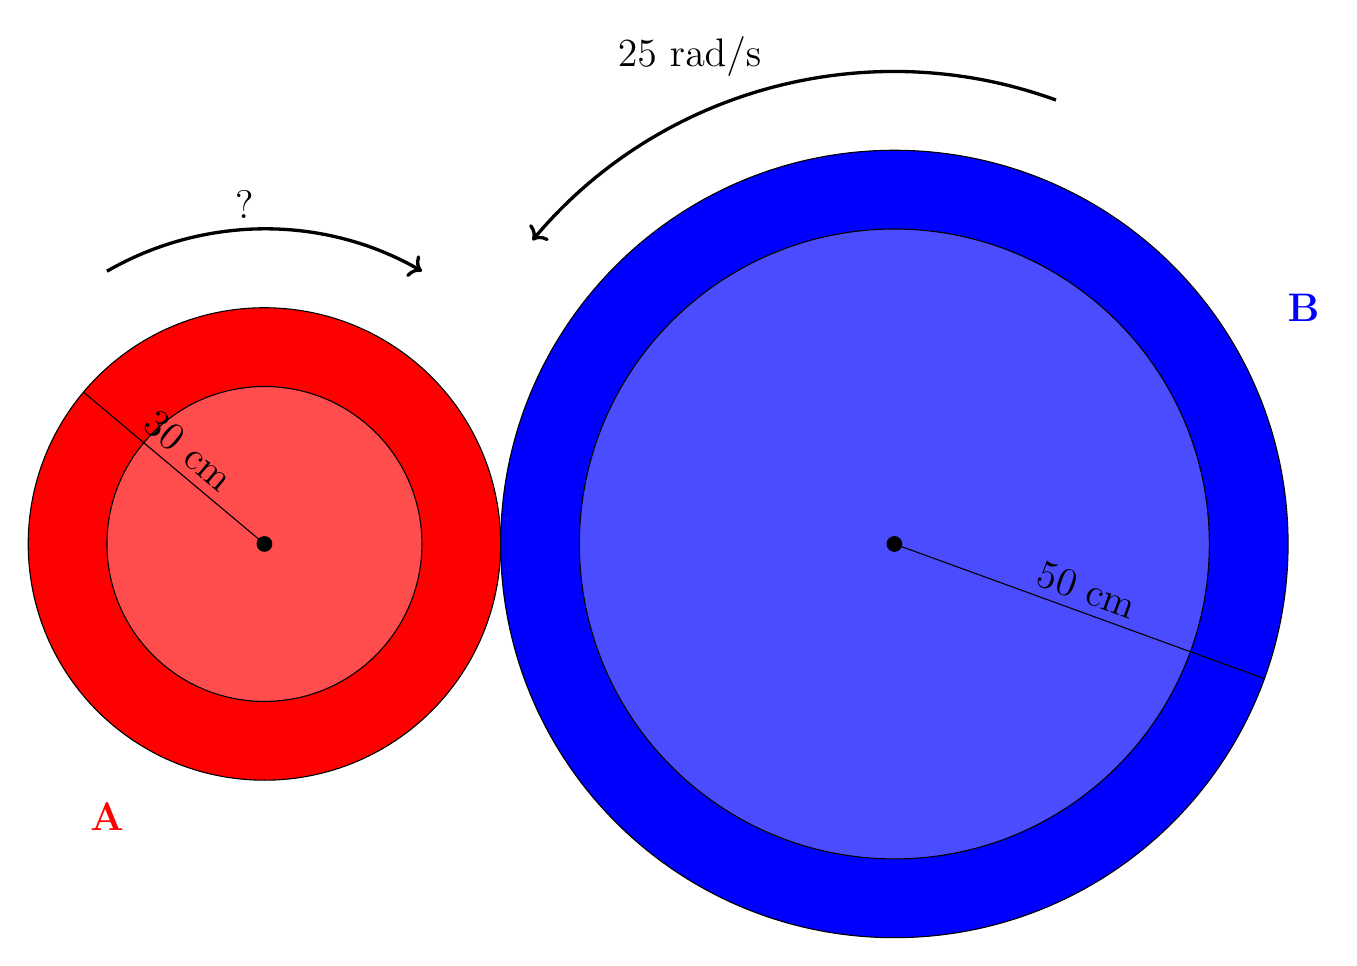
\begin{tikzpicture}
  \draw[fill=red] (0,0) circle (3);
  \draw[fill=red!70] (0,0) circle (2);
  \fill (0,0) circle (0.1);
  \draw[fill=blue] (8,0) circle (5);
  \draw[fill=blue!70] (8,0) circle (4);
  \fill (8,0) circle (0.1);
  \draw[->,very thick] (8,0) ++(70:6) arc (70:140:6)
    node[midway,anchor=south east] {\Large 25 rad/s};
  \draw[->,very thick] (0,0) ++(120:4) arc (120:60:4)
    node[midway,anchor=south east] {\Large ?};
  \draw (0,0) -- ++(140:3) 
    node[midway,sloped, above] {\Large 30 cm};
  \draw (8,0) -- +(-20:5) 
    node[midway,sloped, above] {\Large 50 cm};
  \path (0,0) ++(240:4) node[red] {\Large \bf A};
  \path (8,0) ++(30:6) node[blue] {\Large \bf B};



\end{tikzpicture}
\end{document}